
\vspace{-.05in}
\section{Coloring the Tree}
\label{sec:analysis}
The structure of the \RT provides initial insights about the \MSC that describe the underlying scalar function in terms of the distribution, size, and persistence of the partitions. The expressiveness of the \RT becomes apparent when we encode additional information about the underlying scalar function. In particular, we fit linear models to the data points in each partition and compute various measures that provide insights about the local behaviour of the underlying scalar function within a partition, as well as comparison between different partitions. 

% \subsection{Workflow}
% Examine the tree looking for: 
% \begin{itemize}
%     \item local simplification. how far up the tree can we go simplify the \MSC
%     \item look for partitions with unique behaviour (linear models)
%     \item simplify the tree itself
% \end{itemize}

\subsection{Attributes and Measures}



Each partition has several inherent attributes, such as the number of samples it contains and the persistence levels where it's created. Additional attributes, such as the min and max values of the function within the partition can be precomputed and saved. Precomputing attributes introduce several challenges. First, while some attributes are fast and cheap to compute and store, others, such as inverse regression curves, require substantial time and space, especially if precomputed for all the partitions in a large tree. Second, many partitions may not be of interest for various reasons such as if they were created due to noise in the data, have too few data points, or have a very short lifespan. Since we often filter out or hide these partitions, precomputing their attributes would be a waste of resources. Third, some attributes describe relative measures between partitions, such as between parent and child, that depends on the particular tree. For example, the lifetime of a partition is the difference between the persistence values for the creation on its parent and itself. Fourth, some attributes, such as the bandwidth used in computing reverse regression curves, depend on parameters the user may change during the exploration, and which will require to recompute them on the fly. Finally, we want to empower users to define and modify their own attributes on the fly.

Our solution is to add the notion of a measure, that is, an attribute that is defined by providing a function to compute it rather than providing its value. A measure will be lazily evaluated for a node and the value will be cached in memory, though the user can save the cached values and the measure function to a file and reloaded next time. The use of measure functions, lazy evaluation, and caching are opaque to the rest of the system, which uses them as regular maps of node id to value. Using this approach allows us to define many attributes without the computational costs, as well as add and modify attributes and measures on the fly. When visualizing a Regulus Tree, we only need to ensure the selected measure was evaluated for the visible nodes. 

Often, several measure functions use similar computations, such as fitting a regression model for a given partition and then computing some derived values. We address this by defining the shared computation as a separate measure, which the other measure functions then retrieve rather than call directly. 
% \autoref{fig:attr-def} shows a simple definition of the lifespan measure. The tree parameter enable the measure to retrieve other attributes/measures of the node.

% \begin{lstlisting}[language=Python, float=tb, label=fig:attr-def, caption=Measure definition, aboveskip=\tinyskipamount]
% def lifespan(tree, node):
%     return node.parent.persistence -
%           node.persistence
           
% tree.add_attr(lifespan) # add measure definition to a tree
% \end{lstlisting}

\subsection{Regression Models}
\label{sec:models}
To study the function behaviour, we employ regression analysis to fit local linear models in the various partitions. As a first step we standardize the full dataset by removing the mean and scaling to unit variance.  We fit a model to each partition independently of any neighboring partitions. The main reason is that a partition can be explored in a variety of settings each leading to different sets of neighboring partitions or even none at all (\autoref{sec:simplification}). We do not want the model of a partition to change during the exploration based on indirect actions. 

A linear model is expressed in terms of a set of coefficient, $\beta_i$ such as that $ \tilde{y} = \sum_i^d x_i \beta_i + \beta_0$,
where $\tilde{y}$ is the predicted value and $\beta_0$ is the intercept. A least square regression model is obtained by minimizing the residual sum of squares between the observed and predicted values, 
\[ \min_\beta\| X\beta - Y \|_2^2 \]
To address the potential problem of multicollinearity in the linear regression, which is common in models with large number of parameters, we use Tikhonov regularization, also known as Ridge regression, which constrains the solution by imposing a penalty on the magnitude of the coefficients,
\[ \min_\beta\| X\beta - Y \|_2^2 + \lambda\| \beta \|_2^2 \]
where large $\lambda$ leads to smaller coefficients and a more robust solution to collinearity.

Our attributes and measures approach allows us to accommodate different regression models and freely switch between them during an investigation. We first define a set of model computational functions and then assign one as the current model measure, see \autoref{code:models}. Measures that depend on the regression model in a partition can fetch the 'model' attribute as shown in \autoref{code:fitness}. The model can be replaced at run-time, which in turn invalidates all the models that were already computed, as well as all other measures that depend on it.  

\begin{lstlisting}[language=Python,caption=Using different regression models., 
    float=hbt, label=code:models]
def linear_model(tree, node):
    return LinearRegresssion().fit(node.x, node.y)
def ridge_model(tree, node):
    return Ridge().fit(node.x, node.y)
tree.add_attr(ridge_model, name='model')
\end{lstlisting}

Higher order regression models can also be used although they are more complex and in some sense defeat the purpose because they are not monotonic and it is difficult to interpret their coefficients. High-order model also suffers from the curse of dimensionality; a linear model requires d+1 parameters to describe an d-dimensional data but a quadratic model requires $O(d^2)$ parameters.



\vspace{-.05in}
\subsection{Measures}
\label{sec:measures}

Basic measures we often use include the lifespan, minimum and maximum value, and normalize size. We also define measures to assign a unique id (encoded as different colors) to minima and maxima critical points that are shared between partitions. A shared minima/maxima measure shows the tree from a perspective of merges of minimum/maximum critical points, which in some sense is similar to a merge tree.


\begin{lstlisting}[language=Python, caption=Fitness score (not suitable for derived trees), float=b, label=code:fitness]
def fitness(tree, node):
    model = tree['model'][node]
    return model.score(node.x, node.y)
def parent_fitness(tree, node):
    parent_model = tree['model'][node.parent]
    return parent_model.score(node.x, node.y)  
def child_fitness(tree, node):
    model = tree['model'][node]
    return model.score(node.parent.x, node.parent.y)
\end{lstlisting}

\subsubsection{Fitness}
\label{sec:fitness}
Given a linear regression model for a partition, the first question is how well the linear model actually fits the data. The \MSC guarantees that the data is monotonic within a partition at persistence level 0 but it does not imply linearity. Level 0 partitions that do not have a good linear model fit imply the function was undersampled. At higher persistence levels, multiple partitions with good but different linear models might merge into a single partition with a bad fit (e.g. partitions 0 and 45 in \autoref{fig:fitness}). Identifying such instances can be used to determine to locally choose a persistence value lower than the merged partition. 

We evaluate the fitness of a regression model using \textit{coefficient of determination}:
$R^2 = 1 - \frac{\sum (y - \tilde{y})^2}{\sum (y - \hat{y})^2} $,
where $\tilde{y}$ is the predicted value and $\hat{y}$ is the mean value. The score value range between 1.0 (perfect fit) to $-\infty$. A model that always predicts the expected value of $y$ disregarding the input would have a score of 0. 

\textbf{Example:}
\autoref{fig:fitness} (middle right) shows the \RT of the 2D function from \autoref{fig:regulus-tree}. In this case, we encode the fitness score of the linear model in each partition as color after we clamped it to the range 0 (blue) to 1 (red). The details view, \autoref{fig:fitness} left, shows projections of data points in several selected partitions. 

In general, the higher a partition is positioned alone the vertical axis the lower the fitness score will be (less red) as each merger add more points, which by definition can only reduce the fitness. The numerical value of the current attribute is displayed via a tooltip along with additional information. Partitions 21 and 34 have very good models (0.94 and 0.96 respectively) although they are very different from each other with respect to the $x1$ dimension. This difference is reflected in their parent, partition 20, which has a lower fitness score (0.77) due to the nonlinearity the merge introduced in the $x1$ dimension. 

The shallow hill (top left in the 3d view) contains over half the data points and is captured by partition 45 as a merge of four partitions with very good but very different linear models, leading to a fitness score of only (0.42). Close examination (zooming) confirms that two of the partitions merge first, followed by a merge with the third and fourth. The two intermediate partitions are not stable and have a very short lifespan. Finally, the root of the tree, partition id 0, consists of the entire domain (2000 sample points), and represent the case where we simplify the \MSC all the way down to a single partition. As can be expected, the fitness score is only 0.38 since there is no good global linear model for the data. 


\begin{figure}[bt]
    \begin{center}
     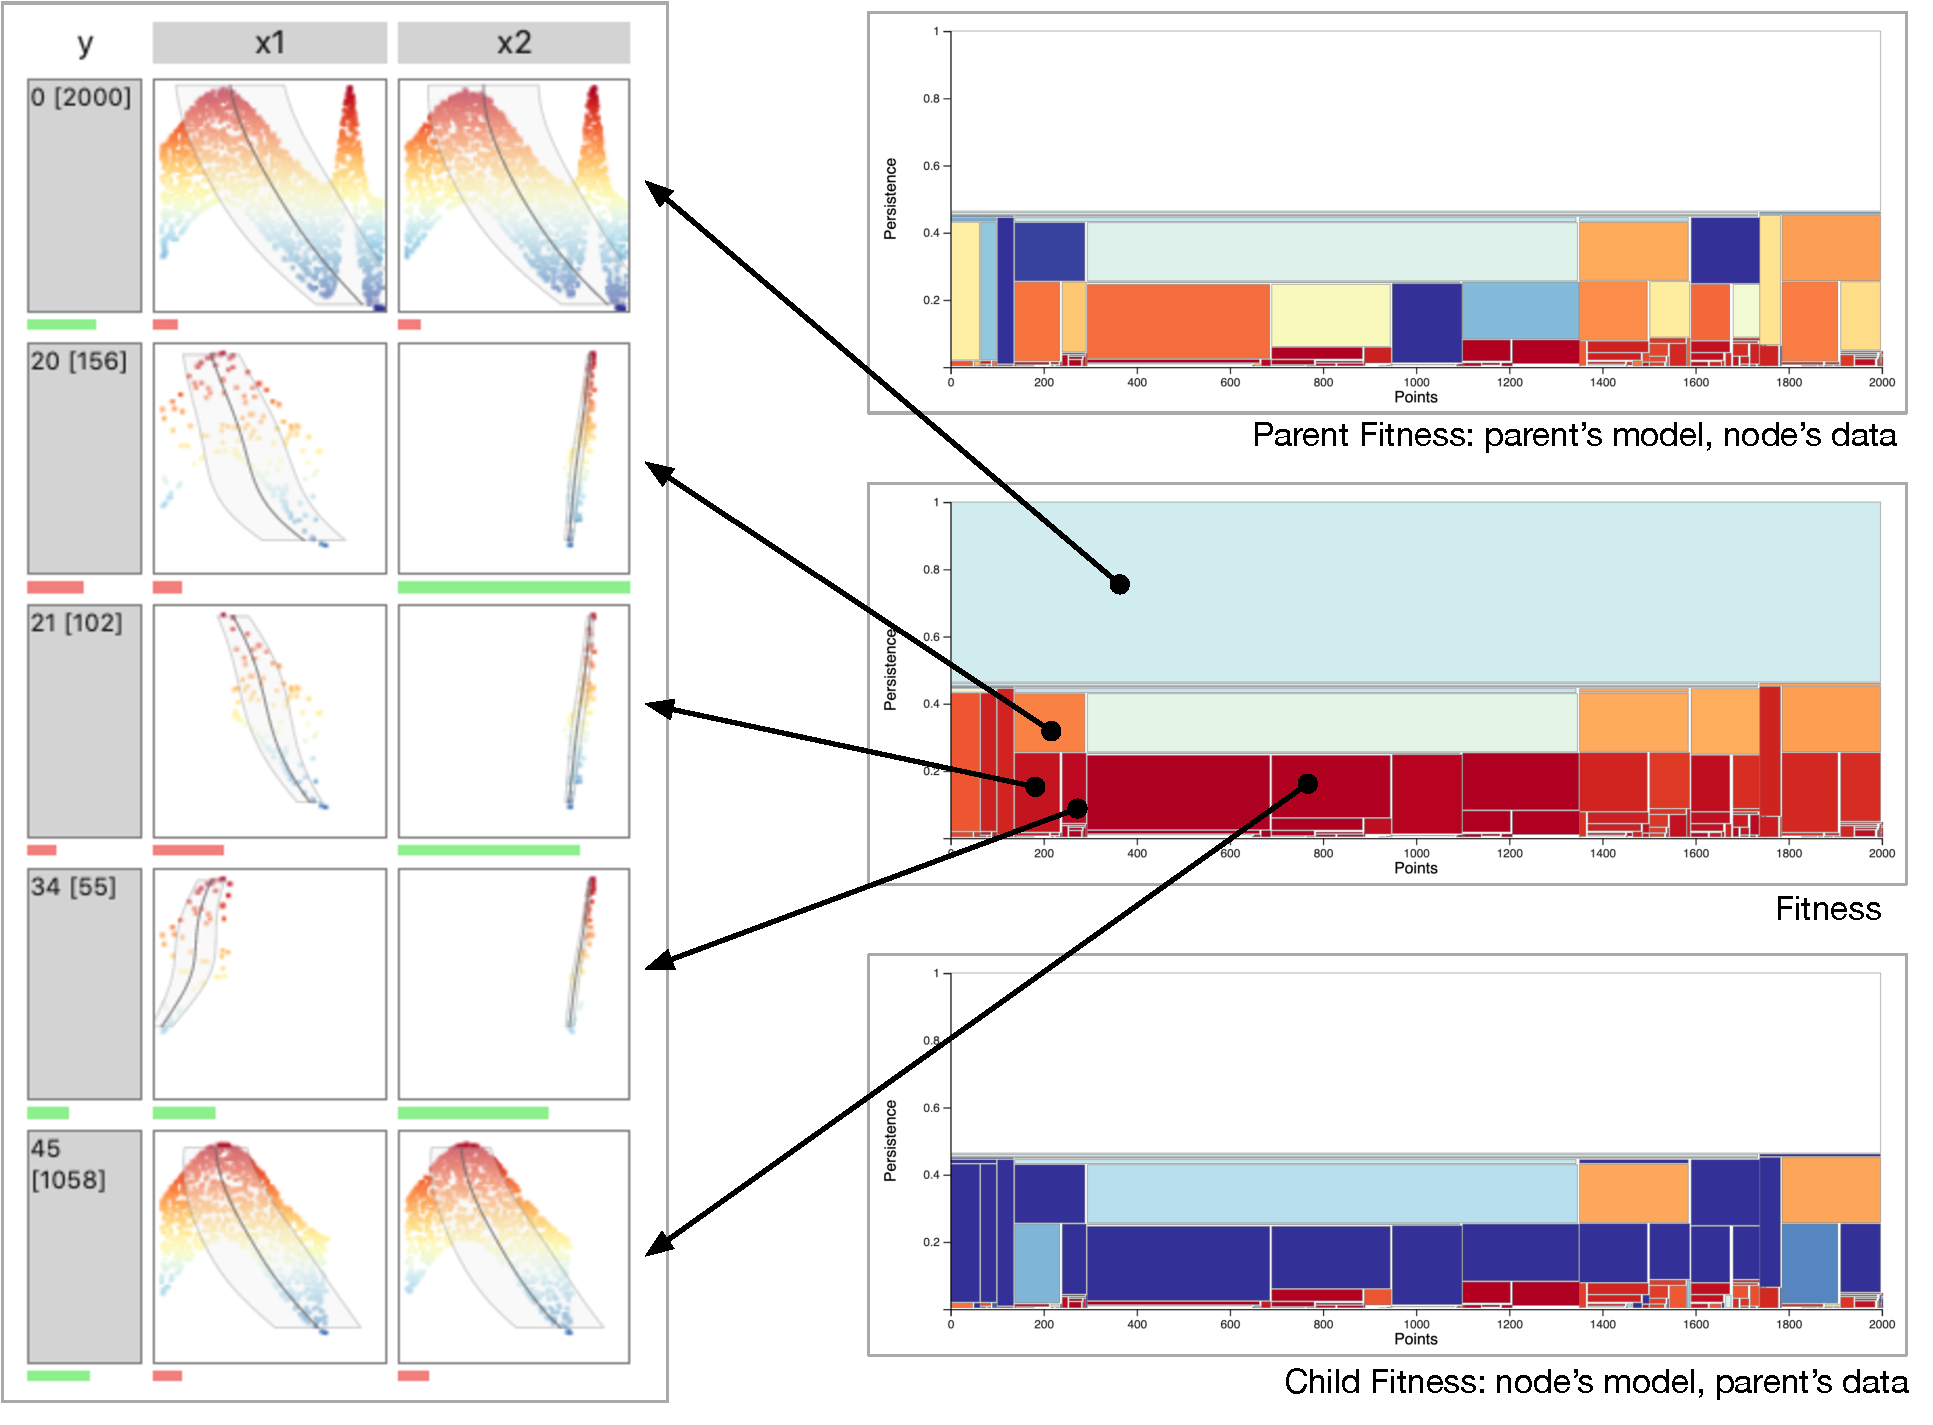
\includegraphics[width=\linewidth]{details-5}
    \caption{Left: details view showing points in selected partitions. Right: Three views of the Regulus Tree, each showing separate fitness measure (blue = 0, red = 1)}
    \label{fig:fitness}
    \end{center}
\end{figure}

\textbf{Parent and Child Fitness}
Partitions 20, 21 and 34 in the above example, highlight the case where a merger of two partitions, both with very good linear models, can lead to a partition with a much worse fitness score. In this case, we should avoid simplifying further at least locally. The different situation can arise where the parent model is very similar one of the children but not the other one. \autoref{fig:fitness-issue}
depict a potential merger between two partitions for a 1d scalar function, where both the children and the parent have good linear models. If we rely only on the fitness score of the parent, we may conclude that the parent represents a good simplification choice, a decision we may not take if we examine at the actual data. This scenario can occur, for example, when one partition contains a lot more data points then the second partition. In some applications, this can be addressed by giving different weights to the points in the two partition. In the context of this work, we specifically want to identify and flag situations like this as they are likely pointing region where the scalar function have unique characteristics. Furthermore, we would like to be able to detect these cases directly in the \RT without the need to examine the data points.
\begin{figure}[b]
    \begin{center}
     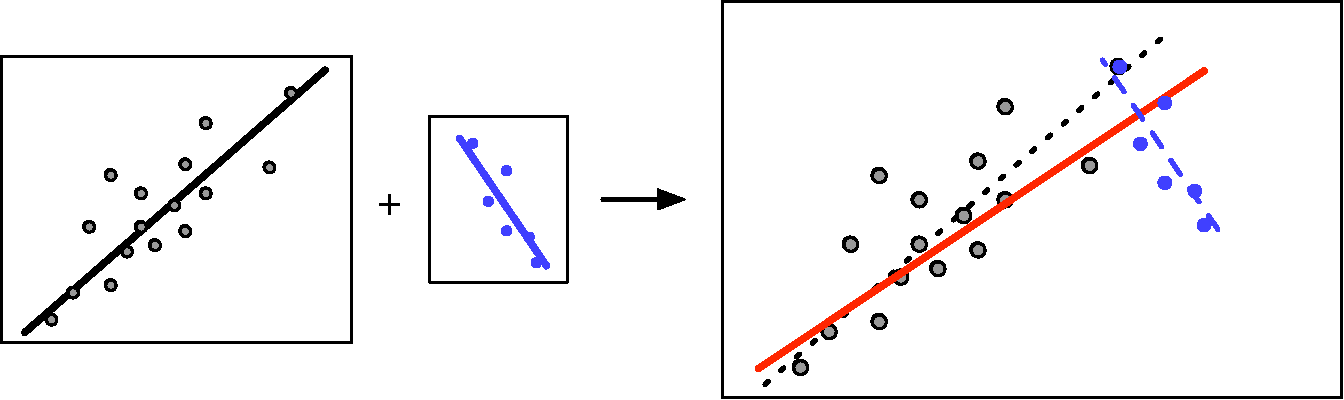
\includegraphics[width=.8\linewidth]{fitness-issue-1}
    \caption{A merge of two partitions with good but different models can lead to a partition with a model that is similar to only one of them.}
    \label{fig:fitness-issue}
    \end{center}
\end{figure}

To address this issue we introduce two \textit{relative} fitness measures as shown in \autoref{code:fitness}. The \textit{Parent Fitness} is the fitness score of the parent's model with respect to the partition data. Conversely, the \textit{Child Fitness} is the fitness score of the partition model with respect the parent's data. Referring back to \autoref{fig:fitness}, the parent fitness is shown in the top right tree and the child fitness in the bottom right tree. The parent fitness indicates that the model of partition 20 moderately fits the data in partitions 21 and 34 (0.79 and 0.65 respectively). The child fitness scores clearly show that the models for partitions 21 and 34 do not fit well with their parent's data (0.2, -1.8 respectively), strongly implying that this simplification step should not be used.



\textbf{Example part II:}
Using the combination of fitness and child fitness scores, we can see that a persistence level of 0.2 provides a very good simplification value. \autoref{fig:graph} shows a top down projection of the full \MSC and both top down and side view projections of the simplified \MSC.  We designed our visual exploration environment specifically to cater to this kind of workflow where multiple measures need to be considered at the same time. The user can visualize multiple \RT instances, each encoding different measures, or simply define a new measure that returns a value based on evaluation of the the fitness, child fitness, and parent fitness in the partition.

\begin{figure}[bt]
    \begin{center}
     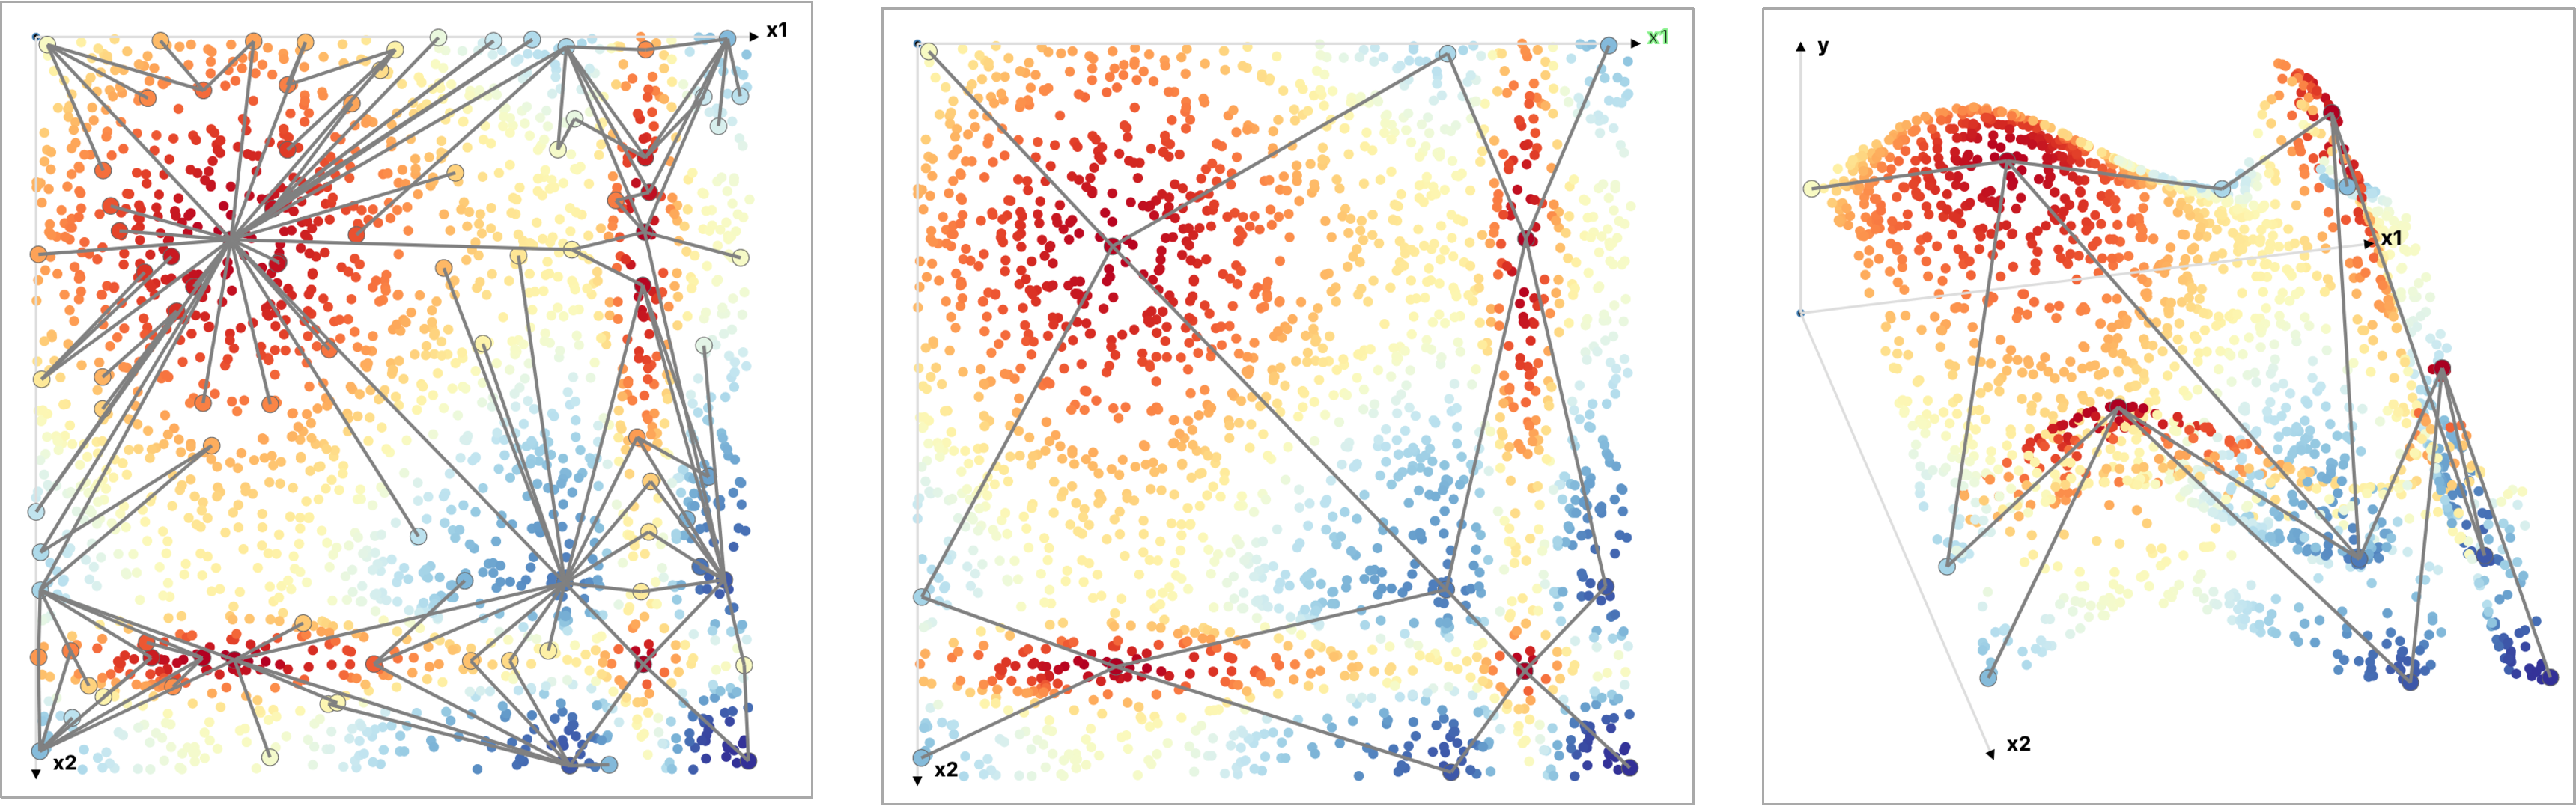
\includegraphics[width=\linewidth]{gauss-graph2}
    \caption{Left: Graph view of the full \MSC and the data points as viewed from above. Middle: Simplification for persistence level = 0.2 Right: Adding the y-axis and slightly rotating the x1- and x2 axis generates a pseudo 3D projection.}
    \label{fig:graph}
    \end{center}
    \vspace{-0.15in}
\end{figure}

\textbf{Reference Model Fitness:}
The parent and child fitness measures play an important role in our workflow despite being limited to only the local neighborhood of a node. As a side note, we do not define a fitness measure between siblings because in the case of derived trees (see \autoref{sec:filtering} a partition can have more than two children. The advantage of the local nature of the parent and child fitness measures is that we can depict each measure over all the nodes in the tree at once. There are cases, however, where we want to compare and contrast models for more distanced ancestors and even between partitions in different parts of the tree (recall that the tree is organized with respect to the list of merges generated using persistence homology not based on local geometry). Depicting many independent global comparisons at once is not possible. Instead, we define a \textit{reference model fitness} measure that applies a reference model to the data in each partition. When the user hovers over the tree we set the reference model to the model of the node under the mouse and reset the cache to cause the values to be recomputed.

% \begin{lstlisting}[language=Python, caption=Fitness score, float=htb, label=code:reference-fitness]
% def reference_fitness(tree, node):
%     reference_model = tree['reference_model']
%     return reference_model.score(node.x, node.y)  
% \end{lstlisting}

\textbf{Dimension Fitness:}
Regression methods fit linear regression models by minimizing cost functions that take into consideration all the dimensions of the data. In that sense the cost (error) is spread over all the dimensions. Within the context of this work, we are trying to identify unique partitions, which means we aim to find maximum discrepancies between partitions and in particular with respect to individual dimensions.

Our \textit{dimension fitness} approach is to compute a vector of regression models for each partition, one per dimension, instead of a single model. Scoring in this case means applying each model in the vector to the data, resulting in a vector of scores instead of one value. Given two partitions, we apply and score the model vector of one partition to both data sets and finally compute the cosine similarity between the two score vectors (\autoref{code:dim-fitness}).

\begin{lstlisting}[language=Python, caption=Dimension Fitness, float=hbt, label=code:dim-fitness]
def relative_dim(tree, models, data):
    return [models[i].score(data.x[i], data.y) 
            for i in range(len(models)]
def child_dim_fitness(tree, node):
    models = tree['dim_models'][node]
    return cosine_similarity(
        tree['relative_dim'][models, node],
        tree['relative_dim'][models, node.parent])
\end{lstlisting}

% \textbf{Coefficients Fitness:} Instead of applying computing $d$ 1-dimensional models for each partition, we can use the coefficients of the regular $d$-dimensional model. In this case, we define the \textit{coefficients fitness} as the cosine similarity between the coefficients of a node's model and the parent's model. Similarly, we define a reference coefficient's fitness as the cosine similarity relative to the global reference node. 
\vspace{-.1in}
\section{Chained Attributes}
\label{sec:chained_attrs}

Since several trees can point to the same collection of partitions, we would have preferred to store attributes in their respective partition to avoid recomputing them for each tree. On the other hand, relative measures are defined with respect to a tree structure and thus should be stored at the nodes. This means that when looking for an attribute or measure for a partition, we need to know where to search for it, which undermine the notion of separation of concerns.
Derived trees, such as when one tree is a simplification of another, add further complication. The new derived tree will most likely have a similar structure to the original tree but will be composed of new nodes. We would rather not have to copy or recompute and instead reuse those relative attributes the are valid for the new tree. 

Our solution is to chain attributes by maintaining a pointer to the attributes of the parent tree. When the value of an attribute is not found in the new tree, we first consult the parent's attributes before computing the value. To avoid recomputing relative measures, we stored such measures using a key consisting of the ids of both partitions. We can then reuse a previously computed value if the same parent-child pair exist in the original tree. To support this we set the node id to its partition id so that keys stays the same in derived trees. \autoref{code:relative} show how we redefine parent and child fitness in terms of a relative measure (compare to \autoref{code:fitness})

\begin{lstlisting}[language=Python, basicstyle=\footnotesize,
    caption=Chained attributes. Parent/child relation depends on the current tree structure, 
    float=tb, 
    breaklines=false,
    label=code:relative]
def relative_fitness(tree, has_model, has_pts):
    return tree['model'][has_model]
           .score(has_pts.x, has_pts.y)
def parent_fitness(tree, node):
    return tree['relative_fitness'][node.parent,node]
def child_fitness(tree, node):
    return tree['relative_fitness'][node,node.parent]    
\end{lstlisting}
